\documentclass[conference]{IEEEtran}
\usepackage[T1]{fontenc}
\usepackage{amsmath}
\usepackage{booktabs}
\usepackage{graphicx}
\usepackage{xcolor}
\usepackage{tikz}
\usetikzlibrary{arrows.meta,positioning,calc}
\usepackage{balance}
\usepackage{stfloats}
\usepackage[hidelinks]{hyperref}
\hypersetup{pdftitle={KVFold: Expanding Cache Capacity for LLM Agents with Lossless Compression},
            pdfsubject={ICDE demonstration review draft, version 14}}
\definecolor{fpInk}{HTML}{172634}
\definecolor{fpBlue}{HTML}{1D62D0}
\definecolor{fpTeal}{HTML}{007E6A}
\definecolor{fpOrange}{HTML}{D96C05}
\definecolor{fpPurple}{HTML}{735892}
\tikzset{
  fpbox/.style={draw,rounded corners=2pt,align=center,inner sep=5pt,
                minimum height=0.73cm,line width=0.65pt},
  fparrow/.style={-{Stealth[length=1.7mm]},line width=0.8pt,draw=fpInk},
  fpboth/.style={{Stealth[length=1.7mm]}-{Stealth[length=1.7mm]},
                 line width=0.8pt,draw=fpInk}
}
\title{KVFold: Expanding Cache Capacity for \mbox{LLM Agents} with Lossless Compression}
\author{\IEEEauthorblockN{Working draft}
\IEEEauthorblockA{Author information to be supplied}}
\raggedbottom
\begin{document}
\maketitle

\begin{abstract}
LLM agents often reuse long prompt prefixes as they continue a task or
resume a session. Caching the corresponding key/value (KV) states avoids
repeated prefill, but cache capacity limits how many requests can run
concurrently and how much history can be retained. KVFold uses lossless
exponent coding to fit more KV into GPU memory and external storage.
Pool mode stores FragPack records on the GPU, decoding them into BF16 for
FlashAttention-3 during prefill and within a fused attention kernel during
decode. Tier mode uses a separate record
format in LMCache and leaves the GPU cache layout and attention
implementation unchanged. In recorded AgentX runs with a fixed 54~GiB KV
budget per GPU, pool mode increases usable capacity from 1.18M to 1.59M
tokens. Visitors can extend and edit a coding-agent prompt to inspect
prefix reuse and KV reconstruction, then explore recorded results showing
how the additional capacity affects concurrent requests and returning
sessions.
\end{abstract}

\section{Introduction}
Consider a coding agent investigating a timeout. Its prompt includes
repository context, a bug report, and the investigation history. When the
user follows the diagnosis with a request for a regression test, most of
the prompt remains unchanged. Prefix caching lets the engine reuse the
keys and values already computed for this shared context, avoiding repeated
prefill. vLLM stores KV in paged blocks~\cite{vllm}, while LMCache retains
reusable prefixes in DRAM and NVMe across requests~\cite{lmcache}.

For Qwen3-30B-A3B, each cached token requires 96~KiB of BF16 KV across all
layers. With many concurrent sessions, requests may have to wait for free
GPU blocks even when their prefixes are available in external storage.
Moving inactive histories to external tiers relieves GPU memory pressure,
but those tiers can also fill up. When a session resumes after its prefix
has been evicted, the engine must recompute that prefix. Cache capacity
thus limits both request concurrency and the amount of history available
for reuse.

KVFold uses lossless compression to fit more KV into the available GPU
memory and external storage. The codec preserves each BF16 value's low
byte, assigns short codes to frequent high-byte values, and uses escapes
for the remaining values. Unlike quantization methods such as
KIVI~\cite{kivi} or lossy context codecs such as CacheGen~\cite{cachegen},
it reconstructs the original KV bits. The main \emph{pool mode} stores
completed GPU blocks as FragPack records. During prefill, KVFold gathers
and decodes the context's KV into a BF16 workspace for FlashAttention-3
(FA3)~\cite{fa3}. During decode, it reconstructs operands within a fused
attention kernel. An alternative \emph{tier mode} stores compressed KV in
LMCache while retaining the native GPU cache layout and attention
implementation. Both modes share the coding principle and offline
calibration, but use different record formats for attention and external
storage.

The demonstration follows the agent as it continues a task, runs alongside
other sessions, and resumes an earlier investigation. Interactive requests
show prefix reuse, external restoration, and KV byte checks.
Recorded AgentX workloads~\cite{agentx} illustrate the effect at scale:
with a 54~GiB KV budget per GPU, pool mode holds 1.59M tokens compared
with 1.18M for the uncompressed baseline. With admission capped at
12 requests, mean engine time to first token (TTFT) falls from 5.16 to
1.94~s, excluding time spent waiting at the proxy.

\begin{figure*}[t]
\centering
% KVFold architecture, manuscript version 5.
% Topology: industry.pdf, Sections III--VI, and manuscript version 3.
% Native vector primitives; oblique depth denotes pages, chips and devices,
% not measured capacity. Blue = FragPack payload; orange = BF16/attention;
% teal = external-cache devices and tier payload. The lanes are alternatives.
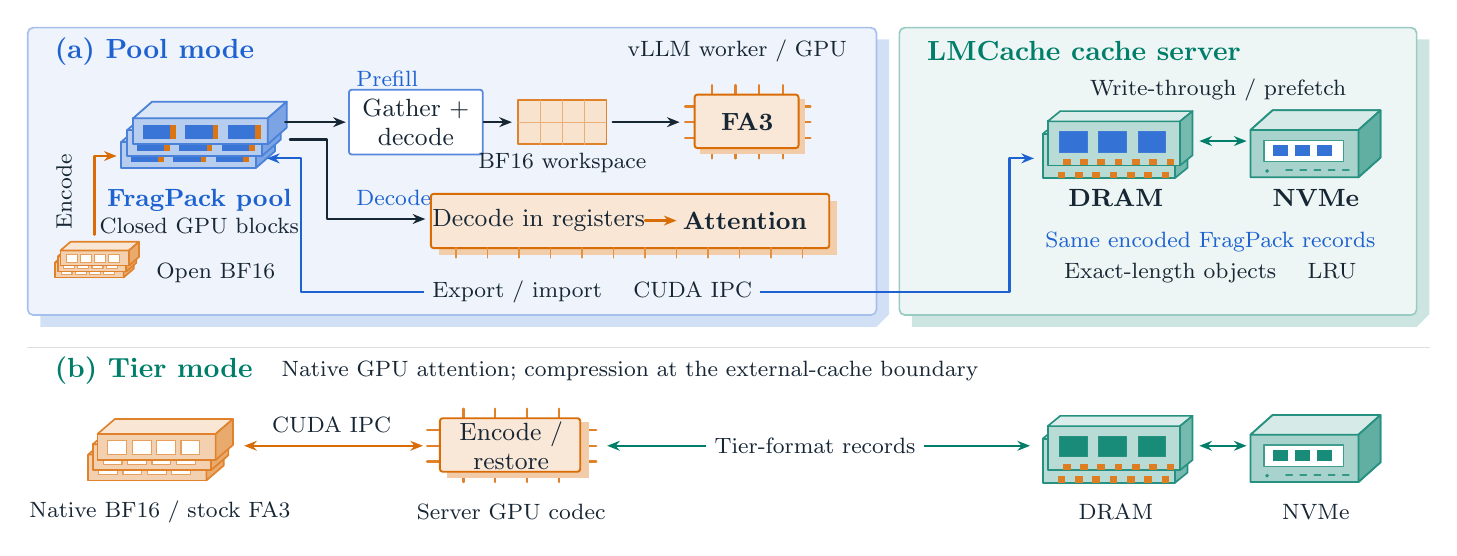
\begin{tikzpicture}[x=1cm,y=1cm,text=fpInk,
    font=\fontsize{9}{10.5}\selectfont,
    line join=round,line cap=round,
    flow/.style={-{Stealth[length=1.6mm,width=1.25mm]},line width=.8pt,draw=fpInk},
    transfer/.style={{Stealth[length=1.6mm,width=1.25mm]}-{Stealth[length=1.6mm,width=1.25mm]},line width=.8pt,draw=fpBlue},
    smalltext/.style={font=\fontsize{8}{9}\selectfont},
    pics/packed/.style={code={
      \foreach \z in {0,.15,.30} {
        \begin{scope}[shift={(.5*\z,\z)}]
          \draw[fpBlue!80,line width=.65pt,fill=fpBlue!32]
            (-.91,-.13) rectangle (.80,.20);
          \draw[fpBlue!80,line width=.65pt,fill=fpBlue!16]
            (-.91,.20) -- (-.67,.41) -- (1.04,.41) -- (.80,.20) -- cycle;
          \draw[fpBlue!80,line width=.65pt,fill=fpBlue!58]
            (.80,-.13) -- (1.04,.08) -- (1.04,.41) -- (.80,.20) -- cycle;
          \foreach \x in {-.79,-.25,.29} {
            \fill[fpBlue!88] (\x,-.06) rectangle +( .35,.17);
            \fill[fpOrange!94] (\x+.35,-.06) rectangle +(.07,.17);
          }
        \end{scope}
      }
    }},
    pics/native/.style={code={
      \foreach \z in {0,.13,.26} {
        \begin{scope}[shift={(.45*\z,\z)}]
          \draw[fpOrange!85,line width=.6pt,fill=fpOrange!32]
            (-.83,-.21) rectangle (.67,.12);
          \draw[fpOrange!85,line width=.6pt,fill=fpOrange!17]
            (-.83,.12) -- (-.61,.31) -- (.89,.31) -- (.67,.12) -- cycle;
          \draw[fpOrange!85,line width=.6pt,fill=fpOrange!58]
            (.67,-.21) -- (.89,-.02) -- (.89,.31) -- (.67,.12) -- cycle;
          \foreach \x in {-.70,-.39,-.08,.23} {
            \draw[fpOrange!65,fill=white,line width=.4pt]
              (\x,-.14) rectangle +(.24,.18);
          }
        \end{scope}
      }
    }},
    pics/chip/.style={code={
      \foreach \x in {-.45,-.15,.15,.45} {
        \draw[fpOrange!85,line width=.9pt] (\x,-.46) -- (\x,-.34);
        \draw[fpOrange!85,line width=.9pt] (\x,.34) -- (\x,.47);
      }
      \foreach \y in {-.20,0,.20} {
        \draw[fpOrange!85,line width=.9pt] (-.79,\y) -- (-.65,\y);
        \draw[fpOrange!85,line width=.9pt] (.65,\y) -- (.80,\y);
      }
      \fill[fpOrange!35] (-.60,-.41) rectangle (.73,.30);
      \draw[fpOrange,line width=.7pt,fill=fpOrange!16,rounded corners=1pt]
        (-.67,-.33) rectangle (.65,.35);
    }},
    pics/dram/.style={code={
      \foreach \z in {0,.16} {
        \begin{scope}[shift={(.40*\z,\z)}]
          \draw[fpTeal!85,line width=.65pt,fill=fpTeal!28]
            (-.84,-.25) rectangle (.84,.31);
          \draw[fpTeal!85,line width=.6pt,fill=fpTeal!14]
            (-.84,.31) -- (-.68,.44) -- (1.0,.44) -- (.84,.31) -- cycle;
          \draw[fpTeal!85,line width=.6pt,fill=fpTeal!54]
            (.84,-.25) -- (1.0,-.12) -- (1.0,.44) -- (.84,.31) -- cycle;
          \foreach \x in {-.69,-.19,.31} {
            \draw[fpPayload!85,line width=.4pt,fill=fpPayload!90]
              (\x,-.08) rectangle +(.35,.26);
          }
          \foreach \x in {-.65,-.43,-.21,.01,.23,.45,.67} {
            \fill[fpOrange!88] (\x,-.25) rectangle +(.10,.08);
          }
        \end{scope}
      }
    }},
    pics/nvme/.style={code={
      \draw[fpTeal!85,line width=.65pt,fill=fpTeal!34]
        (-.72,-.24) -- (.65,-.24) -- (.93,.01) -- (.93,.61)
        -- (-.44,.61) -- (-.72,.36) -- cycle;
      \draw[fpTeal!85,line width=.65pt,fill=fpTeal!16]
        (-.72,.36) -- (-.44,.61) -- (.93,.61) -- (.65,.36) -- cycle;
      \draw[fpTeal!85,line width=.65pt,fill=fpTeal!62]
        (.65,-.24) -- (.93,.01) -- (.93,.61) -- (.65,.36) -- cycle;
      \draw[fpTeal!75,line width=.5pt,fill=white]
        (-.55,-.04) rectangle (.46,.23);
      \foreach \x in {-.44,-.16,.12} {
        \fill[fpPayload!90] (\x,.025) rectangle +(.20,.14);
      }
      \fill[fpTeal!85] (-.51,-.16) circle (.025);
      \foreach \x in {-.27,-.09,.09,.27,.45} {
        \draw[fpTeal!80,line width=.55pt] (\x,-.15) -- +( .08,0);
      }
    }}]
  \path[use as bounding box] (0,0) rectangle (17.8,6.35);
  \colorlet{fpPayload}{fpBlue}

  % Raised host regions: the main reader path stays inside the vLLM worker.
  \fill[fpBlue!20] (.16,2.55) -- (10.78,2.55) -- (10.94,2.71)
    -- (10.94,6.20) -- (.16,6.20) -- cycle;
  \fill[fpBlue!7,draw=fpBlue!40,line width=.6pt,rounded corners=2pt]
    (0,2.70) rectangle (10.78,6.35);
  \fill[fpTeal!20] (11.23,2.55) -- (17.64,2.55) -- (17.80,2.71)
    -- (17.80,6.20) -- (11.23,6.20) -- cycle;
  \fill[fpTeal!7,draw=fpTeal!40,line width=.6pt,rounded corners=2pt]
    (11.07,2.70) rectangle (17.64,6.35);
  \node[anchor=west,font=\fontsize{10}{11}\selectfont\bfseries,text=fpBlue]
    at (.22,6.05) {(a) Pool mode};
  \node[anchor=east,smalltext] at (10.53,6.05) {vLLM worker / GPU};
  \node[anchor=west,font=\fontsize{10}{11}\selectfont\bfseries,text=fpTeal]
    at (11.30,6.05) {LMCache cache server};

  % Persistent compressed records and writable, still-open BF16 storage.
  \pic at (2.10,4.70) {packed};
  \node[font=\fontsize{9}{10}\selectfont\bfseries,text=fpBlue]
    at (2.18,4.16) {FragPack pool};
  \node[smalltext] at (2.18,3.84) {Closed GPU blocks};
  \pic[scale=.58] at (.83,3.30) {native};
  \node[smalltext,anchor=west] at (1.51,3.23) {Open BF16};
  \draw[flow,draw=fpOrange] (.85,3.72) -- (.85,4.72) -- (1.13,4.72);
  \node[smalltext,rotate=90,fill=fpBlue!7,inner sep=2pt]
    at (.46,4.27) {Encode};

  % Prefill explicitly materializes BF16 before unchanged FA3.
  \node[smalltext,text=fpBlue,anchor=west] at (4.05,5.70) {Prefill};
  \draw[flow] (3.27,5.15) -- (4.04,5.15);
  \node[draw=fpBlue!75,fill=white,line width=.65pt,rounded corners=1pt,
    minimum width=1.70cm,minimum height=.64cm,align=center]
    (gather) at (4.93,5.15) {Gather +\\decode};
  \draw[flow] (gather.east) -- (6.15,5.15);
  \draw[fpOrange!85,fill=fpOrange!19,line width=.55pt]
    (6.23,4.87) rectangle (7.35,5.43);
  \foreach \x in {6.51,6.79,7.07}
    \draw[fpOrange!55,line width=.45pt] (\x,4.87) -- (\x,5.43);
  \draw[fpOrange!55,line width=.45pt] (6.23,5.15) -- (7.35,5.15);
  \node[smalltext] at (6.79,4.63) {BF16 workspace};
  \draw[flow] (7.43,5.15) -- (8.28,5.15);
  \pic at (9.14,5.15) {chip};
  \node[font=\fontsize{9}{10}\selectfont\bfseries] at (9.14,5.15) {FA3};

  % The decode alternative reconstructs operands inside the attention kernel.
  \draw[flow] (3.33,4.93) -- (3.80,4.93) -- (3.80,3.92) -- (5.05,3.92);
  \node[smalltext,anchor=west,text=fpBlue] at (4.05,4.19) {Decode};
  \fill[fpOrange!34] (5.22,3.46) rectangle (10.28,4.15);
  \draw[fpOrange,line width=.7pt,fill=fpOrange!17,rounded corners=1pt]
    (5.12,3.55) rectangle (10.18,4.24);
  \foreach \x in {5.44,5.84,6.24,6.64,7.04,7.44,7.84,8.24,8.64,9.04,9.44,9.84}
    \draw[fpOrange!75,line width=.7pt] (\x,3.43) -- (\x,3.55);
  \node at (6.49,3.90) {Decode in registers};
  \draw[flow,draw=fpOrange] (7.84,3.90) -- (8.24,3.90);
  \node[font=\fontsize{9}{10}\selectfont\bfseries] at (9.11,3.90) {Attention};

  % Pool export/import carries the same encoded attention records.
  \draw[transfer] (3.04,4.69) -- (3.47,4.69) -- (3.47,2.99)
    -- (12.47,2.99) -- (12.47,4.69) -- (12.78,4.69);
  \node[smalltext,fill=fpBlue!7,inner sep=3pt]
    at (7.17,2.99) {Export / import \quad CUDA IPC};
  \pic at (13.73,4.69) {dram};
  \pic at (16.25,4.69) {nvme};
  \node[font=\fontsize{9}{10}\selectfont\bfseries] at (13.82,4.19) {DRAM};
  \node[font=\fontsize{9}{10}\selectfont\bfseries] at (16.36,4.19) {NVMe};
  \draw[transfer,draw=fpTeal] (14.88,4.91) -- (15.48,4.91);
  \node[smalltext] at (15.12,5.56) {Write-through / prefetch};
  \node[smalltext,text=fpBlue] at (15.02,3.63) {Same encoded FragPack records};
  \node[smalltext] at (15.02,3.24) {Exact-length objects \quad LRU};

  % Alternative deployment, aligned with the main path's storage devices.
  \colorlet{fpPayload}{fpTeal}
  \draw[fpInk!15,line width=.55pt] (0,2.29) -- (17.8,2.29);
  \node[anchor=west,font=\fontsize{10}{11}\selectfont\bfseries,text=fpTeal]
    at (.22,1.99) {(b) Tier mode};
  \node[smalltext,anchor=west] at (3.10,1.99)
    {Native GPU attention; compression at the external-cache boundary};
  \pic at (1.60,.81) {native};
  \node[smalltext] at (1.68,.20) {Native BF16 / stock FA3};
  \draw[transfer,draw=fpOrange] (2.75,1.04) -- (5.02,1.04);
  \node[smalltext] at (3.86,1.31) {CUDA IPC};
  \pic[xscale=1.35] at (6.14,1.04) {chip};
  \node[align=center] at (6.14,1.04) {Encode /\\restore};
  \node[smalltext] at (6.14,.20) {Server GPU codec};
  \draw[transfer,draw=fpTeal] (7.36,1.04) -- (12.73,1.04);
  \node[smalltext,fill=white,inner sep=3pt] at (10.00,1.04) {Tier-format records};
  \pic at (13.73,.82) {dram};
  \pic at (16.25,.82) {nvme};
  \node[smalltext] at (13.82,.20) {DRAM};
  \node[smalltext] at (16.36,.20) {NVMe};
  \draw[transfer,draw=fpTeal] (14.88,1.04) -- (15.48,1.04);
\end{tikzpicture}

\caption{KVFold's two integration paths. Pool mode stores FragPack records
on the GPU and exports the same records to LMCache. Tier mode keeps the
native GPU cache layout and encodes and restores KV in the cache server.
In both modes, LMCache manages storage in DRAM and NVMe, including eviction,
write-through, and prefetch. Complete blocks are encoded; open blocks retain
BF16 values for updates and attention.}
\label{fig:architecture}
\end{figure*}

\section{System Description}
\label{sec:design}
KVFold integrates with vLLM 0.30 and the multiprocess cache server in
LMCache 0.5.6 (Figure~\ref{fig:architecture}). vLLM schedules requests and
allocates 128-token blocks. LMCache handles external lookup, LRU eviction,
write-through, and prefetch.

\subsection{Compressing closed blocks in the GPU pool}
New KV is written to a BF16 staging buffer as each block fills. At each
layer, the backend writes the new values, computes attention, and encodes
any blocks that are now complete. These records remain immutable in the
layer's compressed pool. Incomplete blocks stay in staging so that later
tokens can be appended.

A FragPack record stores either K or V for one block, layer, and KV head:
128 tokens with 128 dimensions each, or 32~KiB in BF16. Seven frequent
high-byte values have direct three-bit codes. Other values use a four-bit
escape selector to choose among 15 additional values or fall back to a raw
high byte. K and V use separate tables, calibrated for each layer and KV
head. Low bytes are stored unchanged. Dense streams store scalars in the
order required by the attention kernel's threads
(Figure~\ref{fig:record}).

\begin{figure}[t]
\centering
% Restored worked record example from images/figure2(6).tex.
% Identical scalar values, code assignments, field lengths and alignment.
% Original CPU validation: evidence/record-example.json.
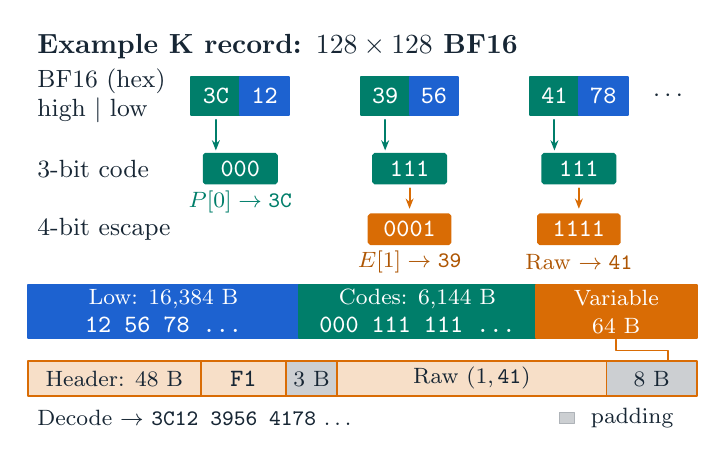
\begin{tikzpicture}[x=1cm,y=1cm,text=fpInk,
    font=\fontsize{9}{10.5}\selectfont,line cap=round,line join=round,
    arrow/.style={-{Stealth[length=1.3mm,width=1mm]},line width=.7pt},
    bits/.style={font=\fontsize{9}{10}\selectfont\ttfamily\bfseries},
    note/.style={font=\fontsize{8.5}{10}\selectfont}]
  \path[use as bounding box] (0,0) rectangle (8.5,5.02);
  \node[anchor=west,font=\fontsize{10}{11}\selectfont\bfseries]
    at (0,4.78) {Example K record: $128\times128$ BF16};

  % Three worked scalars: direct, extended-table and raw escape.
  \node[anchor=west,align=left] at (0,4.15) {BF16 (hex)\\high $\mid$ low};
  \foreach \x/\hi/\lo in {2.70/3C/12,4.85/39/56,7.00/41/78} {
    \draw[fpTeal,fill=fpTeal,line width=.7pt]
      (\x-.62,3.91) rectangle (\x,4.39);
    \draw[fpBlue,fill=fpBlue,line width=.7pt]
      (\x,3.91) rectangle (\x+.62,4.39);
    \node[bits,text=white] at (\x-.31,4.15) {\hi};
    \node[bits,text=white] at (\x+.31,4.15) {\lo};
    \draw[arrow,draw=fpTeal] (\x-.31,3.85) -- (\x-.31,3.46);
  }
  \node[bits] at (8.16,4.15) {$\cdots$};

  \node[anchor=west] at (0,3.23) {3-bit code};
  \foreach \x/\code in {2.70/000,4.85/111,7.00/111} {
    \node[draw=fpTeal,fill=fpTeal,line width=.65pt,
      rounded corners=.7pt,minimum width=.93cm,
      minimum height=.38cm,inner sep=1pt,bits,text=white] at (\x,3.23) {\code};
  }
  \node[note,text=fpTeal] at (2.70,2.81) {$P[0]\to\mathtt{3C}$};

  \node[anchor=west] at (0,2.46) {4-bit escape};
  \foreach \x/\nibble in {4.85/0001,7.00/1111} {
    \draw[arrow,draw=fpOrange] (\x,2.98) -- (\x,2.72);
    \node[draw=fpOrange,fill=fpOrange,line width=.65pt,
      rounded corners=.7pt,minimum width=1.04cm,
      minimum height=.38cm,inner sep=1pt,bits,text=white] at (\x,2.46) {\nibble};
  }
  \node[note,text=fpOrange!80!black] at (4.85,2.05) {$E[1]\to\mathtt{39}$};
  \node[note,text=fpOrange!80!black] at (7.00,2.05) {Raw $\to\mathtt{41}$};

  % Fixed streams show both size and corresponding example data in one band.
  \draw[fpBlue,fill=fpBlue,line width=.7pt]
    (0,1.08) rectangle (3.45,1.75);
  \draw[fpTeal,fill=fpTeal,line width=.7pt]
    (3.45,1.08) rectangle (6.45,1.75);
  \draw[fpOrange,fill=fpOrange,line width=.7pt]
    (6.45,1.08) rectangle (8.50,1.75);
  \node[note,text=white] at (1.725,1.57) {Low: 16,384 B};
  \node[note,text=white] at (4.95,1.57) {Codes: 6,144 B};
  \node[note,text=white,align=center] at (7.475,1.415) {Variable\\64 B};
  \node[bits,text=white] at (1.725,1.25) {12 56 78 \ldots};
  \node[bits,text=white] at (4.95,1.25) {000 111 111 \ldots};

  % Variable-detail pads retain their real byte counts without repeated prose.
  \draw[fpOrange,line width=.6pt] (7.475,1.06) -- (7.475,.92) -- (8.13,.92)
    -- (8.13,.79);
  \draw[fpOrange,fill=fpOrange!22,line width=.65pt]
    (0,.34) rectangle (8.50,.79);
  \fill[fpInk!22] (3.28,.35) rectangle (3.93,.78);
  \fill[fpInk!22] (7.35,.35) rectangle (8.49,.78);
  \foreach \x in {2.20,3.28,3.93,7.35}
    \draw[fpOrange,line width=.5pt] (\x,.34) -- (\x,.79);
  \node[note] at (1.10,.565) {Header: 48 B};
  \node[bits] at (2.74,.565) {F1};
  \node[note] at (3.605,.565) {3 B};
  \node[note] at (5.64,.565) {Raw $(1,\mathtt{41})$};
  \node[note] at (7.925,.565) {8 B};

  \node[anchor=west,note] at (0,.06)
    {Decode $\to$ \texttt{3C12 3956 4178} $\ldots$};
  \fill[fpInk!22,draw=fpInk!35,line width=.4pt] (6.75,-.01) rectangle (6.94,.13);
  \node[anchor=west,note] at (7.03,.06) {padding};
\end{tikzpicture}

\caption{Example of the FragPack record format using illustrative data
(not to scale). The three scalars show direct lookup, an extended-table
escape, and a raw escape. Each raw patch stores an escape's position in
the escape sequence and its original high byte. The variable region uses
64~B in this example, within the format's 2,048~B limit. Recombining the
high and low bytes recovers the original BF16 values exactly.}
\label{fig:record}
\end{figure}

A block's K and V records share a page within each layer. For four KV heads,
a page occupies 190,464~B instead of 262,144~B, allowing the same GPU budget
to hold 1.376 times as many pages before accounting for auxiliary backend
buffers. Records that exceed the encoding limit or do not fit in a shared
page are stored uncompressed in overflow slots.

\begin{samepage}
\subsection{Computing attention from compressed KV}
\emph{Prefill with gather + FA3.} When a request extends the context, the
adapter gathers the context's KV into a BF16 workspace, decoding compressed
records and copying values from open blocks. An unmodified FA3 kernel
computes attention from this workspace, which holds the current layer's KV.
Completed blocks remain compressed in each layer's pool.

\end{samepage}

\emph{Decode with fused attention.} For each generated token, a kernel divides
the request's context into page ranges, prefetches encoded records into
shared memory, and reconstructs operands in registers for tensor-core
attention. A final kernel combines partial softmax states across the
ranges. This path avoids writing the decoded context to GPU global memory
and supports decode-only CUDA graph replay. A vLLM plugin loads the backend
without source changes.

Both paths reconstruct the original KV bits exactly. The console separates
KV byte checks from generated text because fused attention can change
FA3's reduction order.

\subsection{Storing KV in LMCache}
Pool mode exports completed attention records from all layers into a
relocatable blob containing dimensions, table identity, and lengths.
LMCache stores each 128-token block at its actual length in DRAM and NVMe.
On import, records return to GPU pages and their record tables are updated;
failed validation triggers recomputation. The cache server accesses worker
pools through CUDA IPC to run export and import kernels on the corresponding
GPU, with one synchronization per load request.

\emph{Tier mode} preserves the native GPU cache layout and attention
implementation while compressing external KV. Each chunk contains one
block's KV across all layers. Its per-layer, per-head K/V tables share the
pool's calibration but use only 14 symbols, seven primary and seven
secondary, compared with FragPack's 22. Values follow token order. A
three-bit primary code can escape to a second three-bit code and, if
needed, a literal high byte.
Low bytes remain unchanged. FragPack instead uses fragment order and
four-bit escape selectors.
Grouped indices locate escape streams across groups of eight 256-scalar
tiles. Codebooks are fixed
at startup and identified by a table digest. Chunks exceeding the raw
storage limit remain uncompressed.

Each tensor-parallel (TP) rank stores exact-length objects, aligned to
4~KiB for NVMe direct I/O. After the producing step completes, the server
encodes full chunks from native pages into a bounded GPU pool. A background
worker copies and commits the records to DRAM. Loads decode compressed
records into destination pages; raw records and partially shared leading
chunks pass through scratch before scattering. CUDA events order copies,
decoding, and page reuse without host waits on the load path. LMCache uses
stored lengths for NVMe prefetch, allowing the same budget to retain more
history.

\section{Demonstration}
\label{sec:demo}
Visitors follow the timeout investigation through prefix reuse, GPU
pressure, and returning sessions (Figure~\ref{fig:views}). The console
distinguishes live and recorded data and lists the model, TP degree, KV type, mode, and budgets. Modes and codebooks
are fixed at startup; selectors choose saved records.

\begin{figure*}[!b]
\centering
% Interaction-led recomposition of the implemented console and saved evidence.
% Native size 178 x 154 mm. Charts and prefix lengths remain proportional.
% Qwen3-4B interaction/inspector: live-run.json, saved November 8.
% Qwen3-30B AgentX capacity comparisons: paper-evidence.json.
% The inspector overlaps reserved whitespace, not request content or data.
% Its status is a clipped, unmodified native screenshot. The popup-like layout
% is a presentation enlargement, not a claim that the UI implements a modal.
\usetikzlibrary{patterns}
\begingroup
\definecolor{viewInk}{HTML}{222222}
\definecolor{viewRaw}{HTML}{707070}
\begin{tikzpicture}[x=1cm,y=1cm,text=viewInk,
  font=\fontsize{10.5}{12}\selectfont,line cap=round,line join=round,
  every node/.style={inner sep=0pt},
  title/.style={font=\fontsize{12}{14}\selectfont\bfseries},
  note/.style={font=\fontsize{9.5}{11}\selectfont},
  label/.style={font=\fontsize{10.5}{12}\selectfont\bfseries},
  metric/.style={font=\fontsize{11.5}{13}\selectfont\bfseries},
  control/.style={draw=viewInk!45,fill=white,rounded corners=1.5pt,
    minimum height=.50cm,font=\fontsize{10.5}{12}\selectfont},
  flow/.style={-{Stealth[length=1.5mm,width=1.2mm]},line width=.75pt}]
  \path[use as bounding box] (0,0) rectangle (17.8,15.4);

  % (a) A front-facing console window: controls, input, reuse, and answer.
  \draw[viewInk!55,fill=white,rounded corners=2pt,line width=.65pt]
    (.05,5.70) rectangle (16.95,15.35);
  \fill[fpBlue!6,rounded corners=2pt] (.07,14.65) rectangle (16.93,15.33);
  \draw[viewInk!25,line width=.5pt] (.05,14.65) -- (16.95,14.65);
  \node[title,anchor=west] at (.35,15.00) {(a) Prefix reuse};
  \node[note,anchor=east] at (16.60,15.00) {Saved interaction};
  \foreach \x/\label in {2.25/{1. Build},6.35/{2. Append},10.45/{3. Edit early},14.55/{4. Restore}} {
    \node[control,minimum width=3.70cm] at (\x,14.13) {\label};
  }

  % Exact excerpts; line breaks are for paper width, not changed prompt text.
  \draw[viewInk!22,fill=viewInk!2,rounded corners=1.5pt,line width=.5pt]
    (.40,10.08) rectangle (7.55,13.60);
  \node[label,anchor=west] at (.65,13.26) {Prompt excerpt};
  \node[anchor=north west,align=left,font=\fontsize{9.5}{11.3}\selectfont\ttfamily]
    at (.65,12.91) {You are maintaining a Python\\
      repository. Diagnose the timeout\\
      failure below.};
  \node[anchor=north west,align=left,font=\fontsize{9}{11}\selectfont\ttfamily]
    at (.65,11.51) {deadline = monotonic() + timeout\\
      connection = await client.acquire()};

  \node[label,anchor=west] at (7.95,13.35) {Reused / prompt tokens};
  \foreach \x/\col/\lab in {7.95/fpTeal/Reused,10.67/fpBlue/Restored,13.66/fpOrange/Computed} {
    \fill[\col!85] (\x,12.85) rectangle +(.16,.16);
    \node[note,anchor=west] at (\x+.24,12.93) {\lab};
  }
  % One shared 656-token scale; completed steps are a trace, not an animation.
  \foreach \y/\lab/\total/\reuse/\col in {
    12.28/Build/534/0/fpTeal,
    11.63/Append/656/512/fpTeal,
    10.98/{Edit early}/534/0/fpTeal,
    10.33/Restore/534/512/fpBlue} {
    \node[note,anchor=west] at (7.95,\y) {\lab};
    \fill[viewInk!5] (10.05,\y-.13) rectangle +(4.43,.26);
    \draw[fpOrange!80,fill=fpOrange!65,line width=.4pt]
      (10.05,\y-.13) rectangle +({4.43*\total/656},.26);
    \ifnum\reuse>0
      \draw[\col,fill=\col!80,line width=.4pt]
        (10.05,\y-.13) rectangle +({4.43*\reuse/656},.26);
    \fi
    \foreach \k in {1,2,3,4} {
      \draw[white,line width=.6pt] ({10.05+4.43*128*\k/656},\y-.13) -- +(0,.26);
    }
    \node[label,anchor=east] at (16.60,\y) {\reuse\,/\,\total};
  }

  % The rightmost blank part of this panel lies behind the inspector.
  \draw[viewInk!22,fill=white,rounded corners=1.5pt,line width=.5pt]
    (.40,6.02) rectangle (12.05,9.65);
  \node[label,anchor=west] at (.65,9.31) {Model response};
  \node[note,anchor=east,text=fpBlue] at (10.82,9.31) {Restore};
  \node[anchor=north west,text width=9.80cm,align=left,
    font=\fontsize{10.5}{13}\selectfont] at (.65,8.88)
    {The root cause is that the \texttt{timeout} parameter is only used to
    set a deadline for the function's execution, but it is not enforced
    during the \texttt{client.acquire()} call.};
  \draw[viewInk!15,line width=.4pt] (.65,7.02) -- (10.82,7.02);
  \node[anchor=west] at (.65,6.63) {\textbf{512} reused tokens};
  \node[anchor=west] at (4.60,6.63) {TTFT \textbf{47.3 ms}};
  \node[note,anchor=east] at (10.82,6.63) {DRAM $\rightarrow$ GPU};

  % Enlarged independent inspector. This is not a Restore verification path.
  \fill[viewInk!10,rounded corners=2pt] (11.56,5.62) rectangle (17.78,9.97);
  \draw[fpTeal!75,fill=white,rounded corners=2pt,line width=.75pt]
    (11.43,5.75) rectangle (17.65,10.10);
  \fill[fpTeal!7,rounded corners=2pt] (11.45,9.48) rectangle (17.63,10.08);
  \draw[fpTeal!30,line width=.5pt] (11.43,9.48) -- (17.65,9.48);
  \node[title,anchor=west] at (11.70,9.79) {KV Inspector};
  \node[note,anchor=west] at (11.70,9.14) {Independent export/import check};
  \node[note,anchor=west] at (11.70,8.72) {Block 1 $\cdot$ 128 tokens $\cdot$ 36 layers};
  \node[note] at (12.67,8.25) {BF16};
  \node[note] at (15.69,8.25) {Encoded blob};
  \node[metric] at (12.67,7.83) {18.00 MiB};
  \draw[flow,fpTeal] (13.80,7.83) -- (14.50,7.83);
  \node[metric] at (15.69,7.83) {12.73 MiB};
  % Original native screenshot: viewport in pixels (= bp at its native 72 dpi).
  % Pixel rectangle [60,275,760,425], origin at the image's upper left.
  \node at (14.54,6.98) {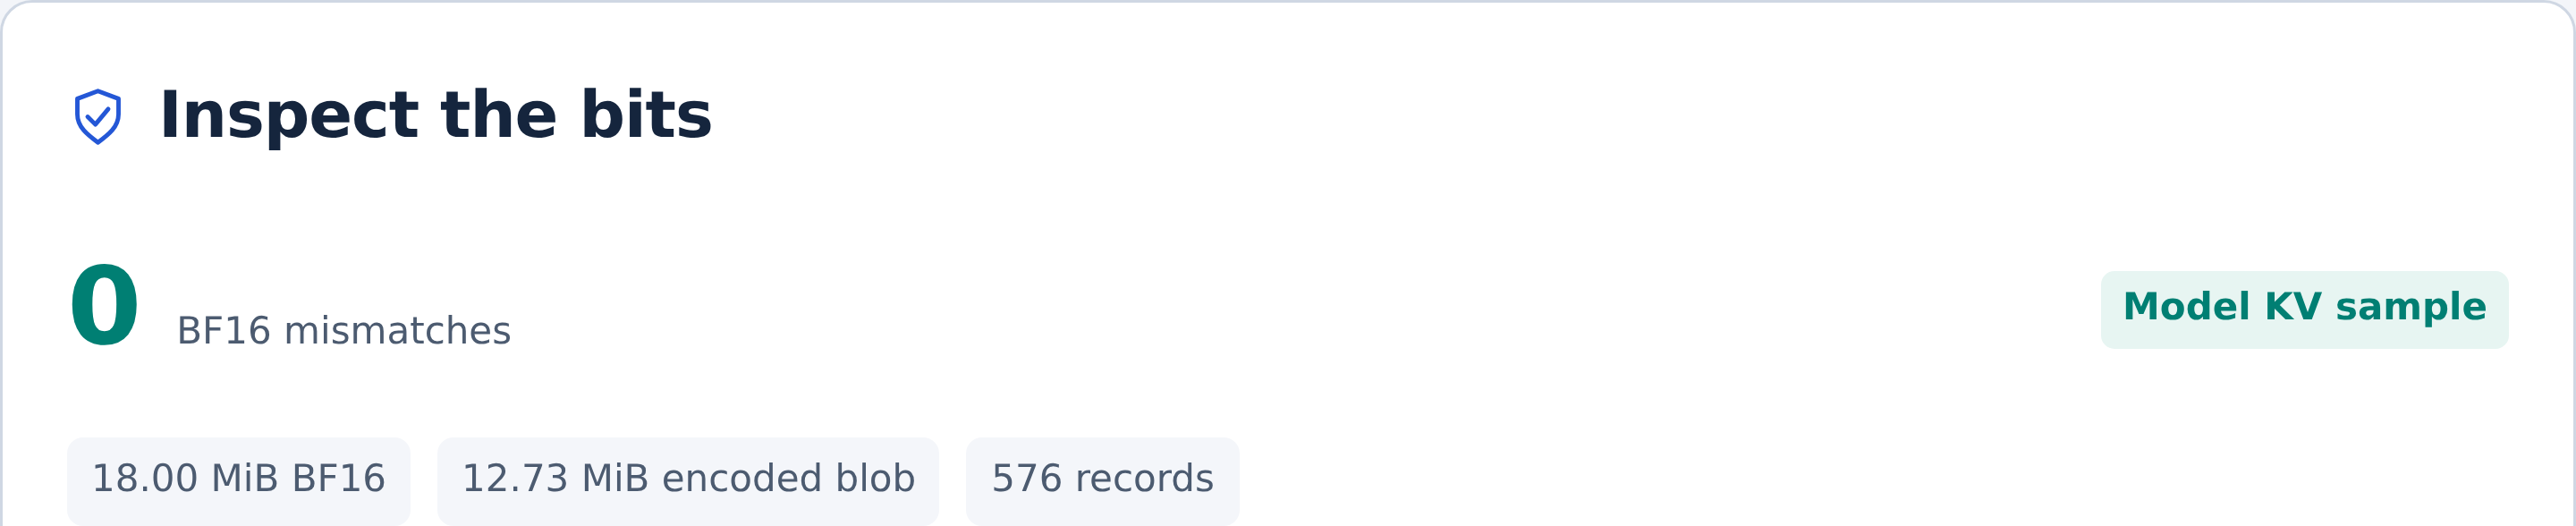
\includegraphics[viewport=60 163 760 313,clip,width=5.30cm]
    {images/console-inspector-recorded(9).png}};
  \node[note,anchor=west] at (11.70,6.12) {After Build $\cdot$ 576 records};

  % (b)(c) Compact, flat archive viewers: configuration and one central chart.
  \foreach \x in {.05,9.10} {
    \draw[viewInk!55,fill=white,rounded corners=2pt,line width=.6pt]
      (\x,.08) rectangle +(8.65,5.05);
  }
  \node[title,anchor=west] at (.35,4.75) {(b) GPU capacity};
  \node[note,anchor=east,text=viewRaw] at (8.40,4.75) {Recorded};
  \node[anchor=west] at (.35,4.11) {Admission};
  \node[control,minimum width=1.45cm] at (5.12,4.11) {$S=8$};
  \node[control,draw=fpBlue,fill=fpBlue!7,minimum width=1.65cm]
    at (7.35,4.11) {$S=12$};
  \node[label,anchor=west] at (.35,3.48) {KV tokens / GPU};
  \node[note,anchor=east] at (8.40,3.48) {54 GiB budget};
  \foreach \y/\lab/\val/\disp/\col in {
    2.82/Raw/1.18/1.18M/viewRaw,2.19/Pool/1.59/1.59M/fpBlue} {
    \node[anchor=west] at (.35,\y) {\lab};
    \fill[viewInk!4] (1.65,\y-.15) rectangle +(5.15,.30);
    \draw[\col,fill=\col!20,line width=.6pt]
      (1.65,\y-.15) rectangle +({5.15*\val/1.6},.30);
    \node[metric,anchor=east] at (8.40,\y) {\disp};
  }
  \draw[viewInk!15,line width=.4pt] (.35,1.67) -- (8.40,1.67);
  \node[note,anchor=west] at (.35,1.19) {Waiting requests (mean)};
  \node[anchor=east] at (8.40,1.19) {1.5 $\rightarrow$ \textbf{0.4}};
  \node[note,anchor=west] at (.35,.61) {Engine TTFT (s)};
  \node[anchor=east] at (8.40,.61) {5.16 $\rightarrow$ \textbf{1.94}};

  \node[title,anchor=west] at (9.40,4.75) {(c) History retention};
  \node[note,anchor=east,text=viewRaw] at (17.45,4.75) {Recorded};
  \node[anchor=west] at (9.40,4.11) {NVMe};
  \node[control,draw=fpTeal,fill=fpTeal!7,minimum width=1.95cm]
    at (13.75,4.11) {640 GiB};
  \node[control,minimum width=1.65cm] at (16.35,4.11) {2 TiB};
  \node[label,anchor=west] at (9.40,3.48) {Cached tokens (GPU + external)};
  \foreach \y/\lab/\val/\col in {2.82/Raw/55/viewRaw,2.19/Tier/91/fpTeal} {
    \node[anchor=west] at (9.40,\y) {\lab};
    \fill[viewInk!4] (10.70,\y-.15) rectangle +(5.15,.30);
    \draw[\col,fill=\col!20,line width=.6pt]
      (10.70,\y-.15) rectangle +({5.15*\val/100},.30);
    \node[metric,anchor=east] at (17.45,\y) {\val\%};
  }
  \draw[viewInk!15,line width=.4pt] (9.40,1.67) -- (17.45,1.67);
  \node[note,anchor=west] at (9.40,1.19) {Stored / raw bytes};
  \node[anchor=east] at (17.45,1.19) {\textbf{71.6\%}};
  \node[note,anchor=west] at (9.40,.61) {Engine TTFT (s)};
  \node[anchor=east] at (17.45,.61) {6.76 $\rightarrow$ \textbf{2.34}};
\end{tikzpicture}
\endgroup

\caption{Console views recomposed for display.
(a) Saved November 8 Qwen3-4B interaction with prefix strips on the same
token scale. The enlarged, repositioned inspector includes a native
screenshot detail; its model-block export/import check is independent of Restore. (b) GPU capacity and
(c) history retention: selectors choose archived Qwen3-30B AgentX
configurations. Cached-token share includes GPU and external cache hits.}
\label{fig:views}
\end{figure*}

\emph{Setup.} The interactive session uses Qwen3-4B-Instruct-2507 with BF16
weights and KV, TP 1, and one H800 PCIe GPU. It uses eager execution in pool
mode, with 128-token blocks, a 4~GiB GPU KV budget, and 1~GiB of LMCache DRAM.

The recorded capacity experiments used Qwen3-30B-A3B-Instruct
with FP8 weights and BF16 KV, TP 2, and two H800 SXM GPUs connected over
PCIe. vLLM used 128-token blocks and 8,192-token chunked prefill.
AgentX harness 1.0.7 replayed \texttt{cc\_traces\_weka\_062126\_256k} with
seed 42 and recorded think times. $P$ counts live root sessions; a FIFO
proxy admits at most $S$ concurrent requests. Measurements covered
1,800 seconds after priming and ten warmup requests, excluding requests
without a first token by the window's end. \emph{Engine TTFT} excludes
proxy wait. \emph{Goodput} counts requests/minute with engine TTFT at most
2~s and inter-token latency (ITL) at most 40~ms.

% Current codec description: feat/lmcache-056-lossless-kv at d096273.
% Recorded measurements: main(11).pdf, November 4, 2026; exact run commits
% are not identified in the supplied report.
These measurements and output checks predate the shared calibration and
grouped index described in Section~\ref{sec:design}. The recorded tier runs
used per-plane codebooks and the earlier tile index.

\subsection{Step 1: extend a task and inspect prefix reuse}
Visitors use \emph{Build} to submit repository context, a bug report,
and ``Diagnose the timeout failure.'' They then \emph{Append} ``Write a
regression test.'' A prefix strip shows reused and new tokens alongside cached-token
counts, TTFT, and the continuation. \emph{Edit early} limits reuse to complete
128-token blocks before the changed token.

\emph{Restore} waits for external saves, resets the GPU prefix cache, and
replays the original prompt. The saved session restored 512 tokens from
LMCache DRAM.

The inspector compares decoded KV from an already encoded block before
and after export through host memory and import into an independent GPU
scratch store, showing sizes, checksums, and mismatch counts. All layers
of the captured 128-token block matched byte for byte. Separate CPU samples
exercise escapes and raw fallback.

A historical check found identical greedy outputs for 192 repeat-trace
requests in tier and raw-tier modes with matching execution paths.

\subsection{Step 2: explore GPU capacity limits}
Visitors switch between $S=8$ and $S=12$ to compare raw and pool modes
under equal GPU KV budgets (Table~\ref{tab:gpu}). The external tiers retain
the working set, with cached-token share fixed at 0.94. These runs examine
GPU pressure when prefixes are already cached.

% Source: main(11).pdf, p.10, Table V; printed values retained verbatim.
\begin{table}[t]
\centering
\caption{GPU capacity and performance in the recorded runs: 54 GiB KV per
GPU, $P=64$, 400 GiB DRAM, and 2 TiB NVMe. Wait denotes the mean number of
requests waiting in vLLM; TTFT is mean engine TTFT in seconds.}
\label{tab:gpu}
\small
\setlength{\tabcolsep}{3pt}
\begin{tabular*}{\columnwidth}{@{\extracolsep{\fill}}rlrrrr@{}}
\toprule
$S$ & Mode & KV tokens & Wait & TTFT & Goodput \\
\midrule
8  & Raw  & 1.18M & 0.3 & 1.69 & 15.1 \\
8  & Pool & 1.59M & 0.2 & 1.34 & 16.2 \\
12 & Raw  & 1.18M & 1.5 & 5.16 & 10.6 \\
12 & Pool & 1.59M & 0.4 & 1.94 & 14.9 \\
\bottomrule
\end{tabular*}
\end{table}

Pool mode reserves 1.3~GiB within the KV budget for staging, overflow, and
the prefill workspace. Cache-server CUDA contexts and transfer buffers are
accounted for separately; codec buffers occupy 1.0~GiB per GPU outside
vLLM's budget.

At $S=12$, pool mode keeps TTFT close to the raw baseline at $S=8$,
while reducing waiting requests and increasing goodput at the same
admission cap.

\subsection{Step 3: revisit sessions under storage pressure}
Visitors switch between 640~GiB and 2~TiB NVMe to compare retained
history, stored bytes, TTFT, and goodput (Table~\ref{tab:tiers}). Raw and tier
modes use the same native GPU KV layout, FA3, and LMCache LRU, write-through,
and prefetch policies; the allocated record sizes differ.

% Source: main(11).pdf, p.9, Table III; same P/S and metric definitions.
\begin{table}[t]
\centering
\caption{External cache capacity and performance in the recorded runs:
$P=64$, $S=8$, and 400 GiB DRAM. Cached denotes the share of prompt tokens
served from the GPU or external cache; TTFT is mean engine TTFT in seconds.}
\label{tab:tiers}
\small
\setlength{\tabcolsep}{3pt}
\begin{tabular*}{\columnwidth}{@{\extracolsep{\fill}}llrrr@{}}
\toprule
NVMe & Mode & Cached & TTFT & Goodput \\
\midrule
640 GiB & Raw  & 0.55 & 6.76 & 4.6 \\
640 GiB & Tier & 0.91 & 2.34 & 13.5 \\
2 TiB   & Raw  & 0.94 & 1.69 & 15.1 \\
2 TiB   & Tier & 0.94 & 1.85 & 15.4 \\
\bottomrule
\end{tabular*}
\end{table}

At 640~GiB NVMe, tier mode's compressed-to-raw size ratio of 0.716 allows
about 1.4 times as much KV to fit (Table~\ref{tab:tiers}). At 2~TiB, the raw
working set fits and cached-token shares converge. Tier input throughput
is then 26.9 thousand tokens/s versus 27.5 for raw storage, a 2.2\% reduction.

A separate replay of 48 prompts, with one request in flight, compares DRAM
and NVMe hits. Their KV occupies 261~GiB raw and 188~GiB compressed. At
220~GiB DRAM, compressed KV fits in memory, while some raw prefixes require
NVMe reads. For 8K--128K prompts, raw storage has 1.63--1.68 times the mean
warm TTFT of tier mode. At 400~GiB DRAM both fit and the gap narrows.
The console displays these recorded residency and latency comparisons.

\section{Conclusion}
KVFold fits more KV into GPU memory and external cache tiers. Visitors
inspect prefix reuse, restore KV from LMCache, and check a model block
before and after transfer. Recorded comparisons show how the additional
capacity affects request queues and history reuse under fixed budgets.

\section*{Acknowledgment}
OpenAI Codex assisted with drafting and figure preparation. Experimental
values were taken from the authors' recorded results.

\bibliographystyle{IEEEtran}
\bibliography{references}
\end{document}
